\subsection{L1L1 cuts}

The cut on the track quality $\chi^2$ is shown in Figure~\ref{fig:trkChi2}. Here, we cut on the individual positron and electron track qualities requiring a $\chi^2$ to be less than 30. 
\begin{figure}[H]
  \centering
      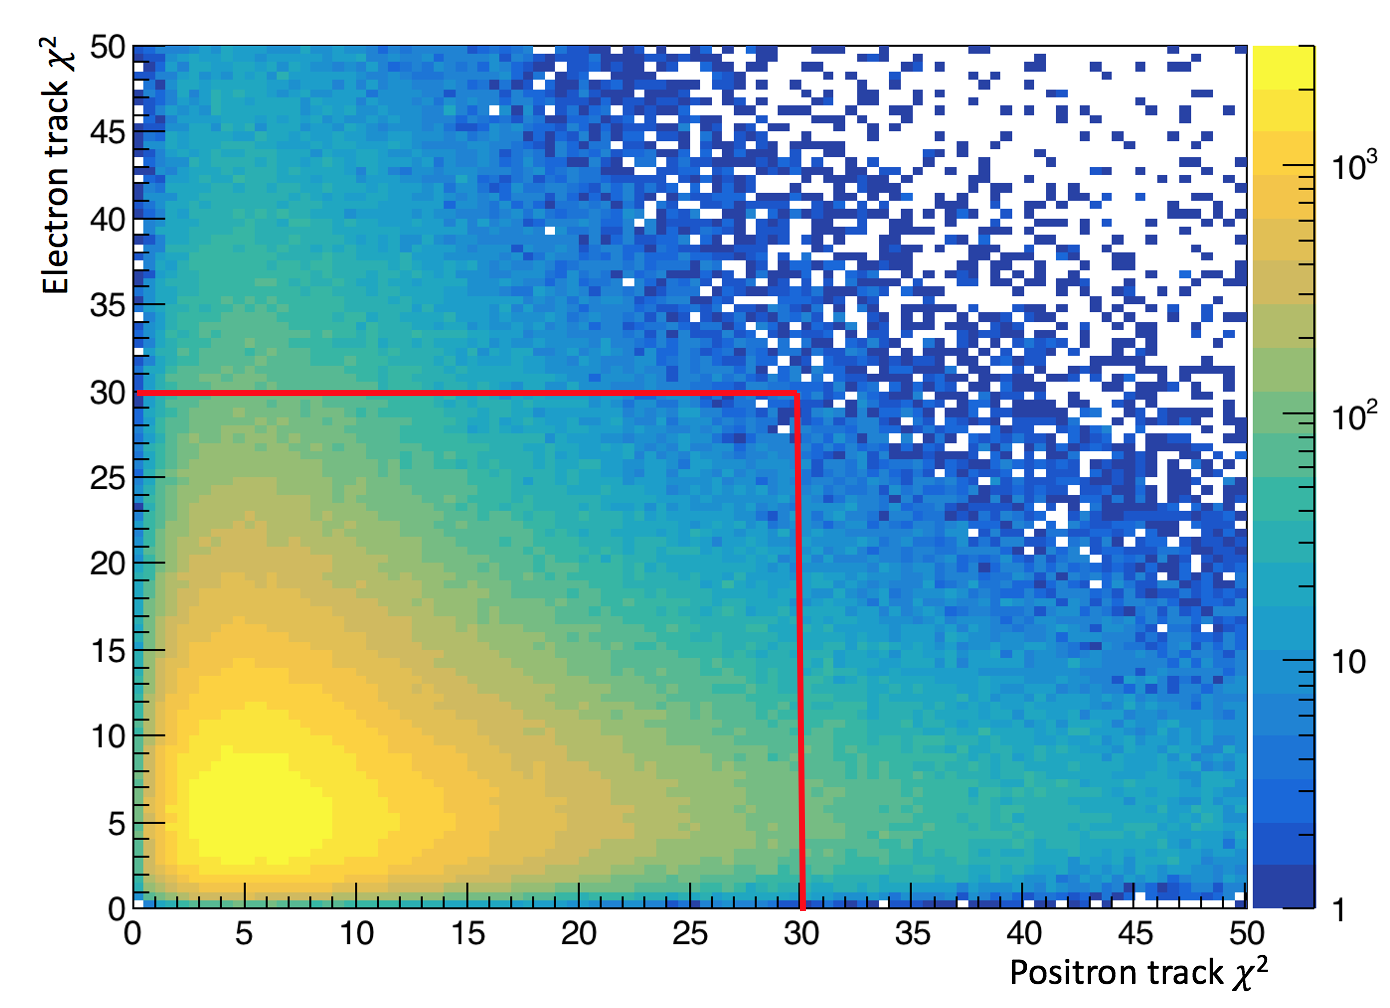
\includegraphics[width=0.65\textwidth]{pics/searching/trkChi2.png}
  \caption[Track $\chi^2$ cut]{The electron and positron track $\chi^2$ are shown with the cut indicated by the red line. This cut is an initial track selection quality cut and uses no vertex or timing information.}
  \label{fig:trkChi2}
\end{figure} 
The cut on the maximum electron track momentum is intended to reduce contamination from elastically-scattered electrons and to correspond to the range of electron energy expected from trident events.  The cut is shown in Figure~\ref{fig:emTrkPmax}.
\begin{figure}[H]
  \centering
      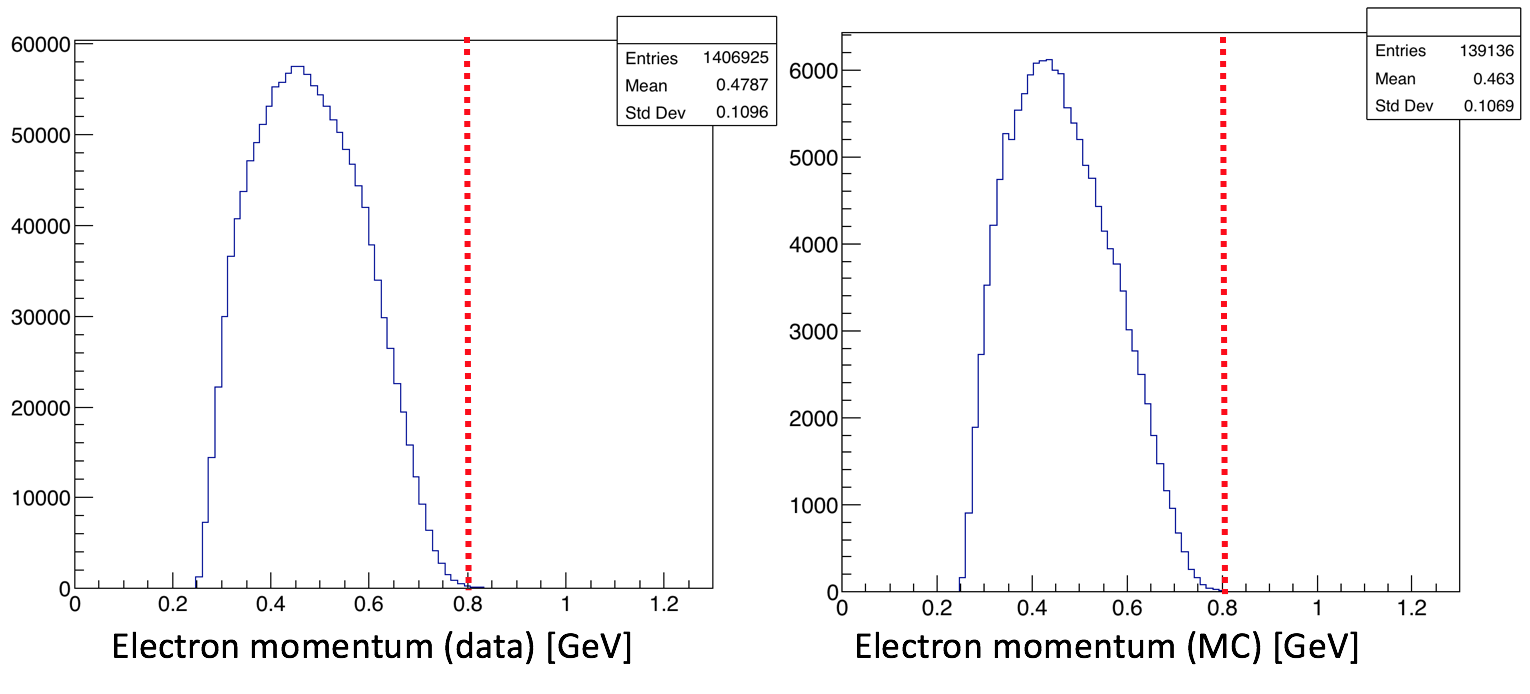
\includegraphics[width=0.65\textwidth]{pics/searching/emTrkPmax.png}
  \caption[Maximum $e^-$ track momentum]{The maximum momentum of the electron track as shown in data (prior to cutting) and Monte Carlo. Events with higher electron energies are attributable to other types of backgrounds in the data such as elastics and wide angle bremsstrahlung and not the trident background.}
  \label{fig:emTrkPmax}
\end{figure} 
A cut to the cluster time difference is set at $\pm$2~ns. This includes events from two beam buckets as shown in Figure~\ref{fig:cltdiff}.
\begin{figure}[H]
  \centering
      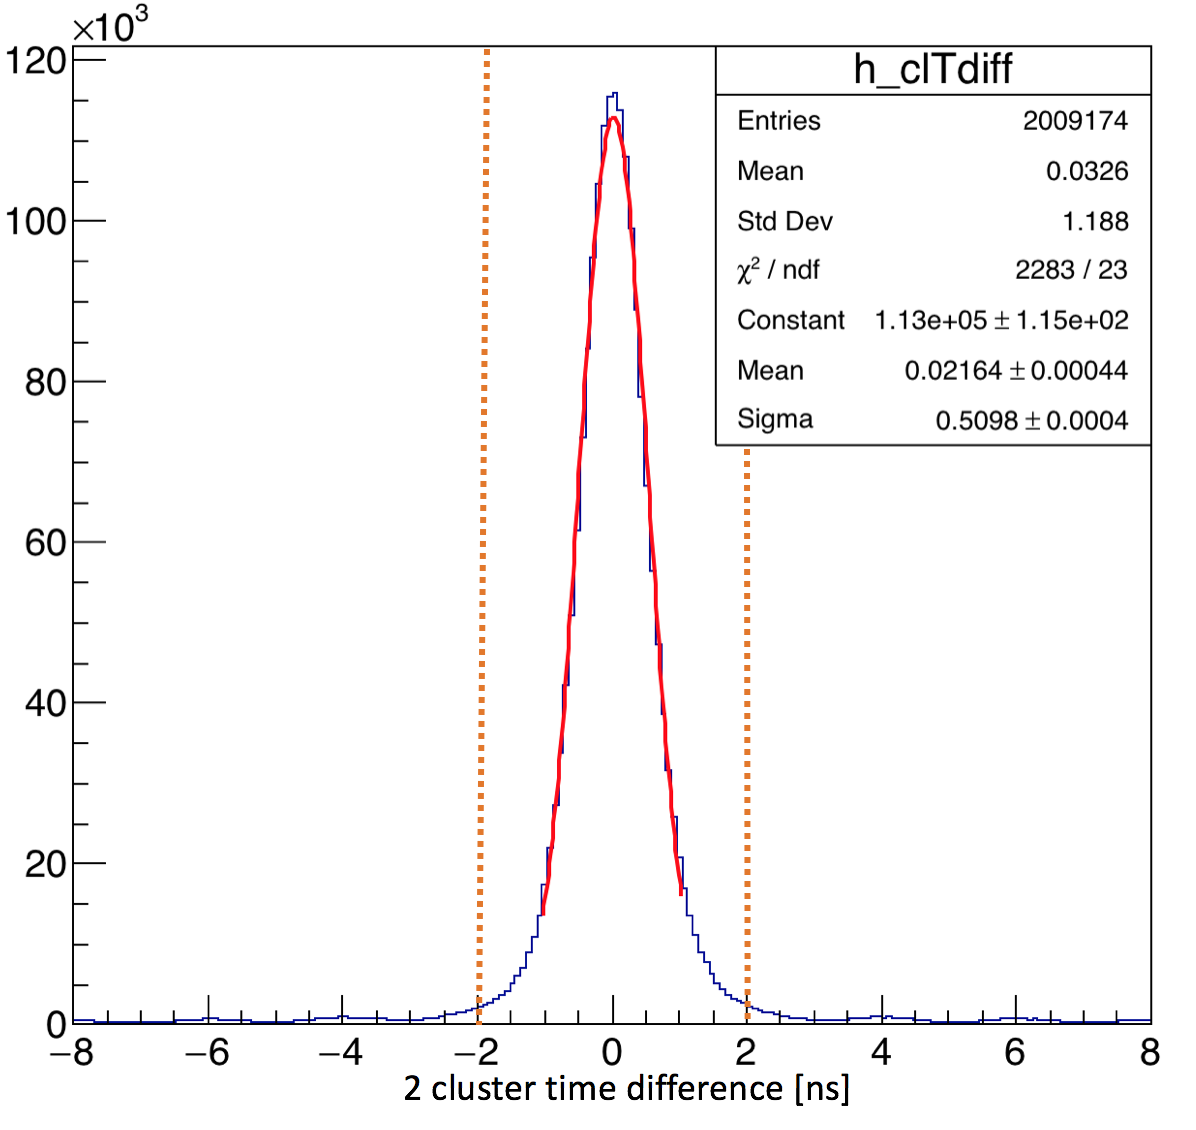
\includegraphics[width=0.6\textwidth]{pics/searching/cltdiff.png}
  \caption[Cut on the cluster pair time difference]{The two cluster timing difference is shown with a fit to the Gaussian central part of the distribution. Additional smaller peaks can be seen in intervals of 2~ns in the tails of the distribution. The timing cut can remove these events where the electron and positron come from different events.}
  \label{fig:cltdiff}
\end{figure} 
The difference between the unconstrained and beam spot constrained vertex $\chi^2$ shows how well a vertexed $e^+e^-$ pair's total momentum projects back to the beam spot position at the target. The cut is shown in Figure~\ref{fig:bmucut}.
\begin{figure}[H]
  \centering
      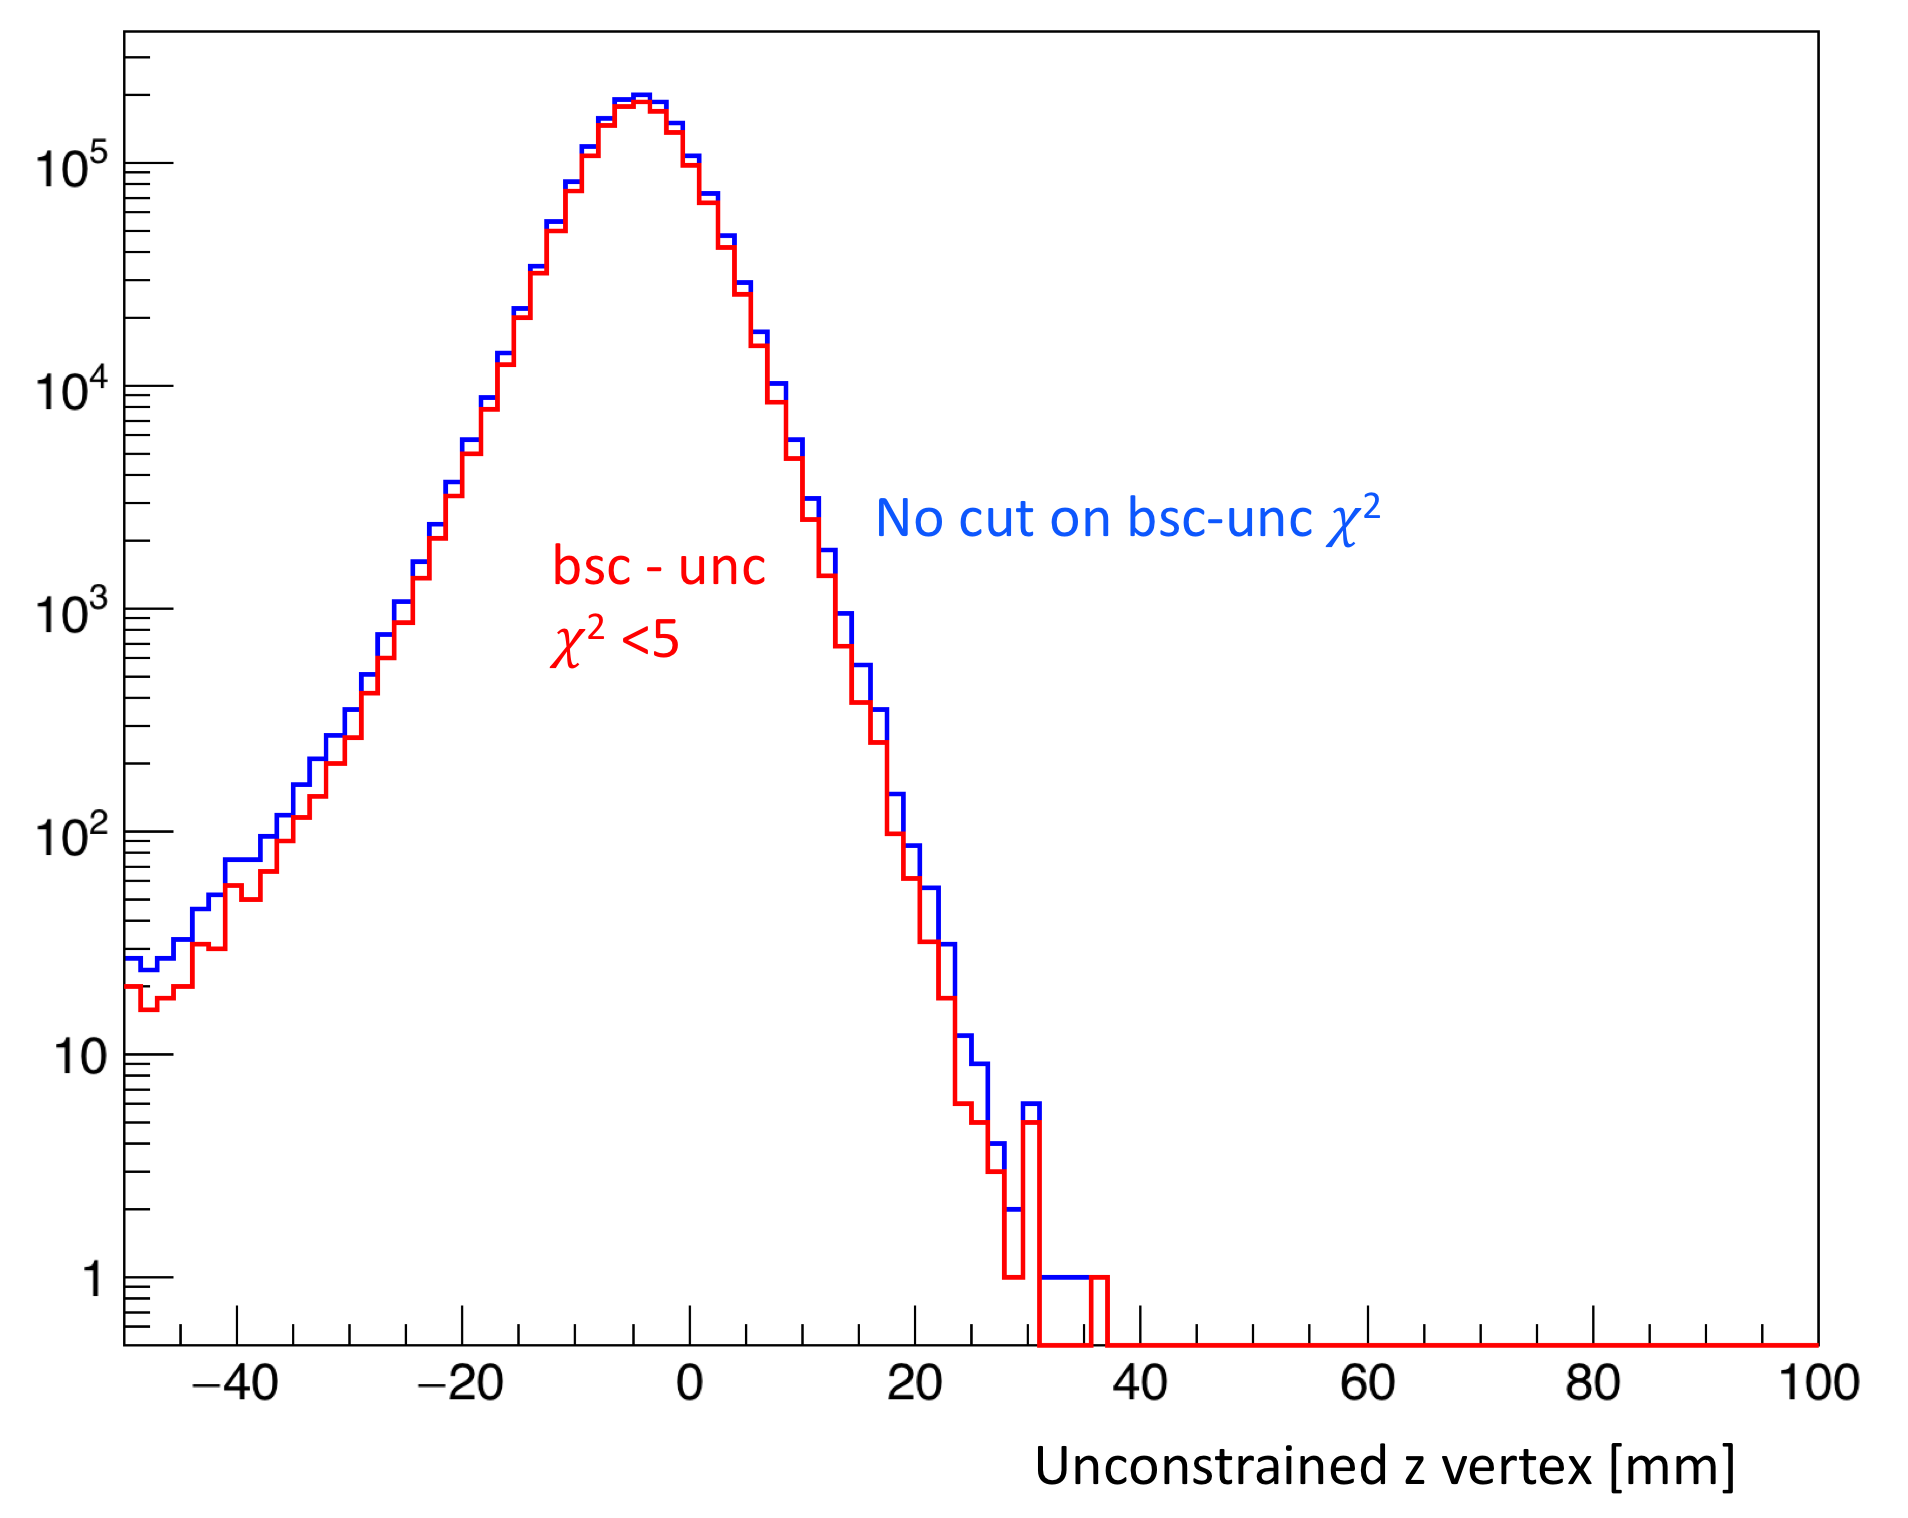
\includegraphics[width=0.45\textwidth]{pics/searching/bmuchi2.png}
  \caption[Vertex cut on the difference between beamspot and unconstrained $\chi^2$]{The effect of a cut on the difference between the beamspot and unconstrained constrained $\chi^2$ on the vertex distribution for all masses. The effects of the cut on the downstream tails of the distribution tells us how well a vertexed pair of tracks points back to the beamspot position at the target.}
  \label{fig:bmucut}
\end{figure} 
The cut to SVT tracks matched to ECal clusters is shown in Figure~\ref{fig:matchcut}. The matching parameter was derived empirically from data and corresponds to the number $\sigma$, derived from the distribution difference of the projected track to the ECal and ECal cluster positions. 
\begin{figure}[H]
  \centering
      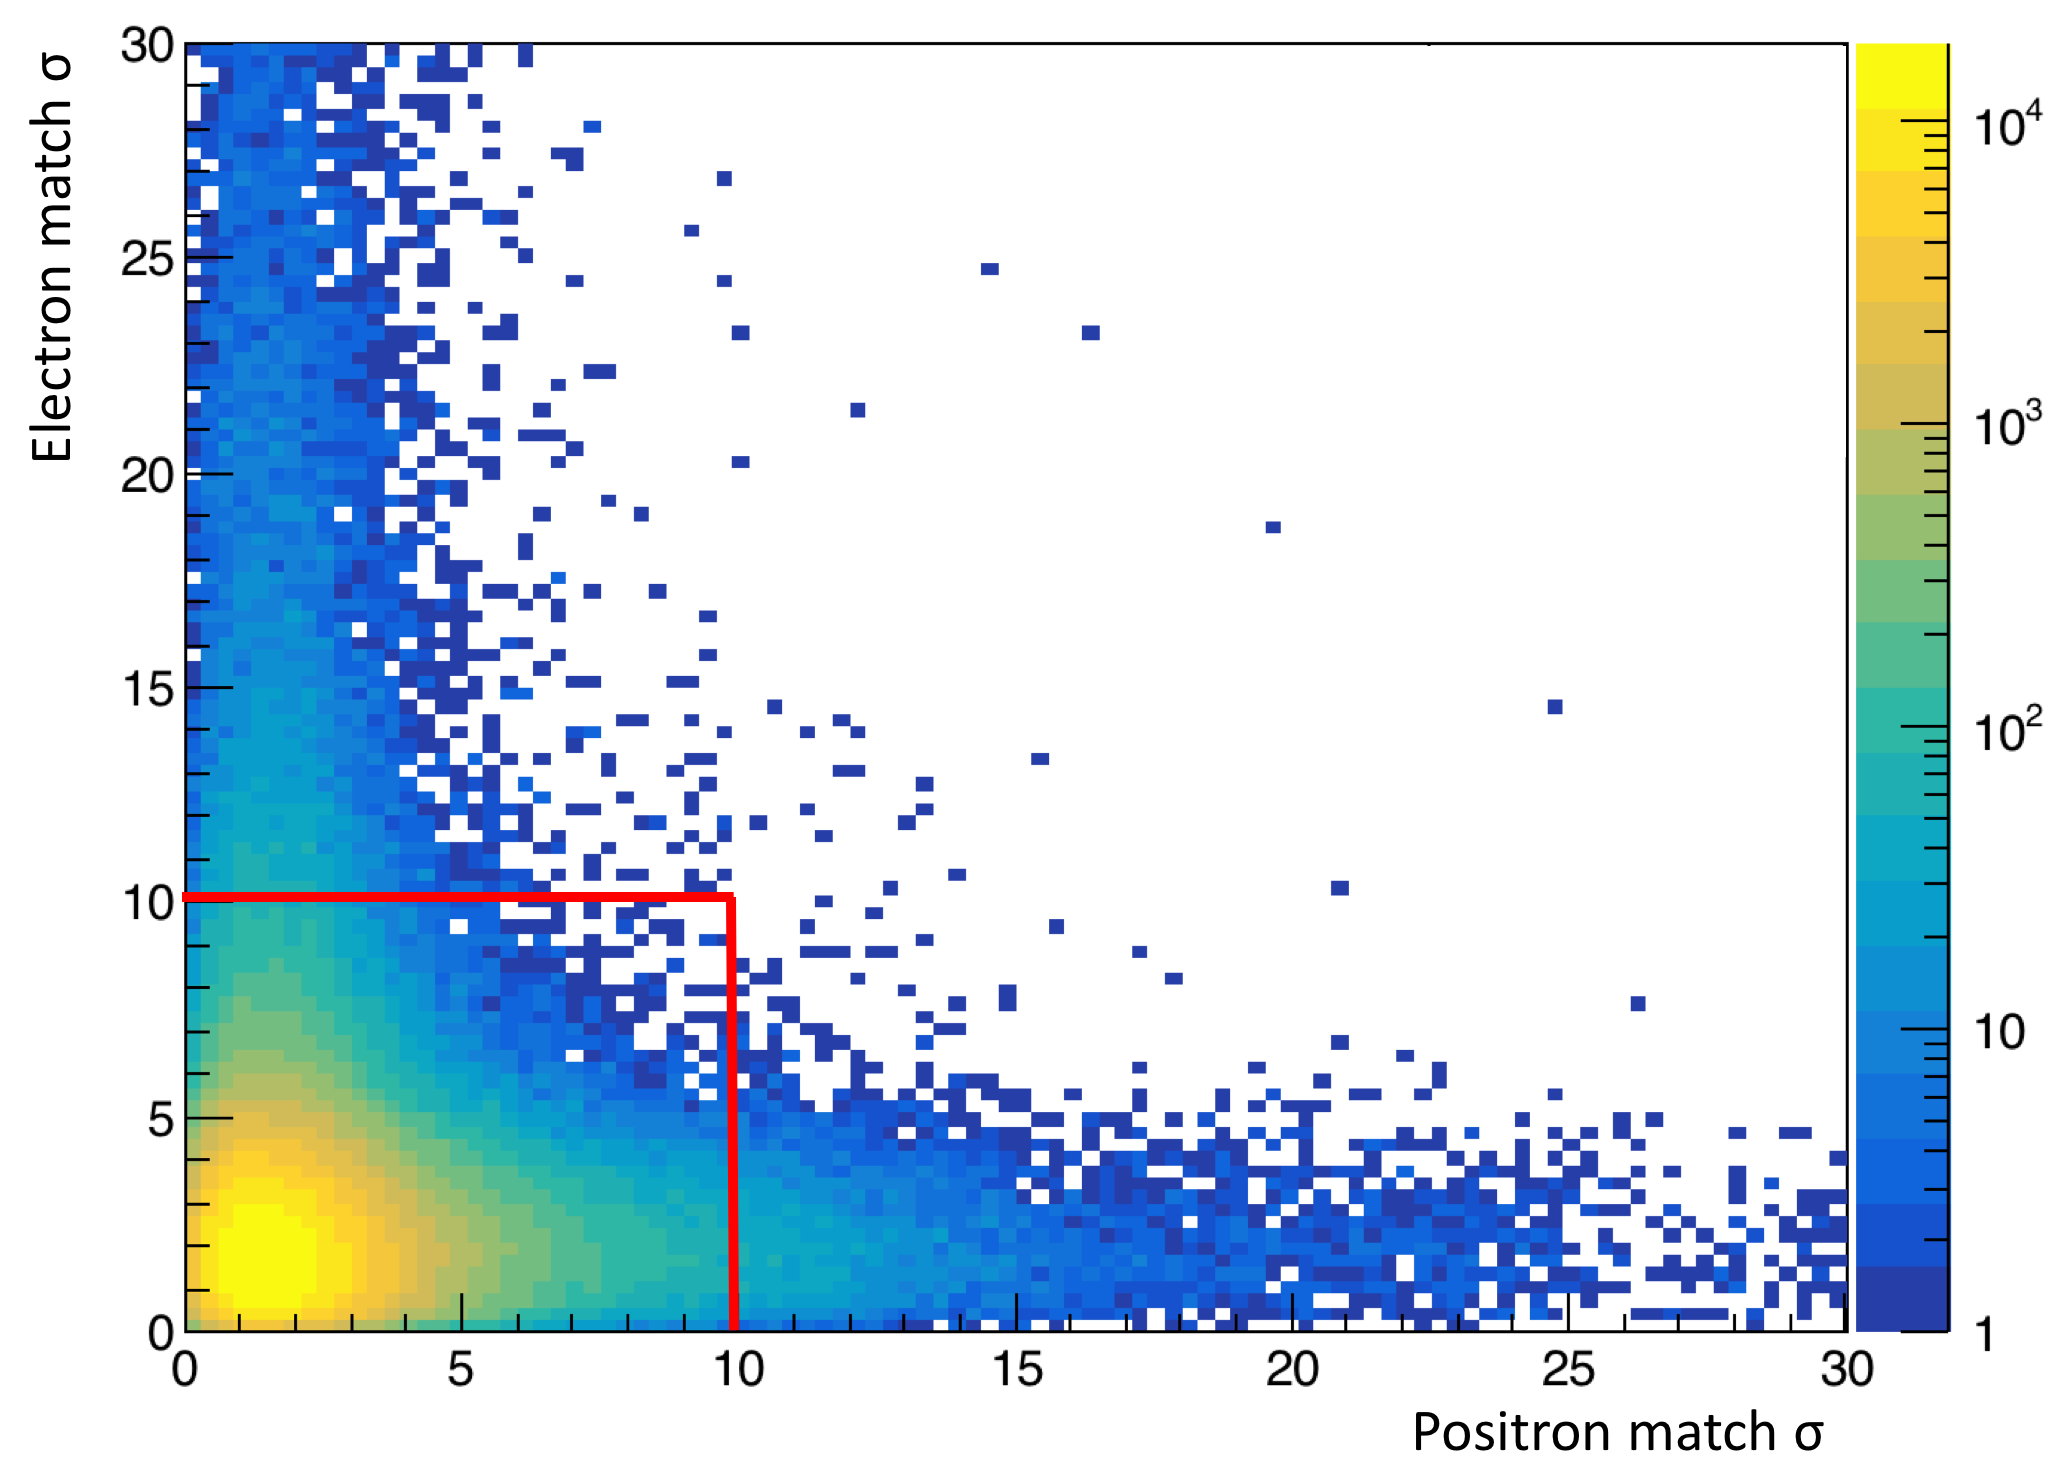
\includegraphics[width=0.45\textwidth]{pics/searching/matchcut.png}
  \caption[Cut on the track-cluster matching]{The SVT track to ECal cluster matching parameter for both electrons and positrons is shown.}
  \label{fig:matchcut}
\end{figure}
The momentum asymmetry cut is defined as the momentum difference over the momentum sum of the $e^+e^-$ tracks. The momentum symmetry is intended to reduce the background WAB contamination. The effects of the cut are shown in Figure~\ref{fig:pasycut}.
\begin{figure}[H]
  \centering
      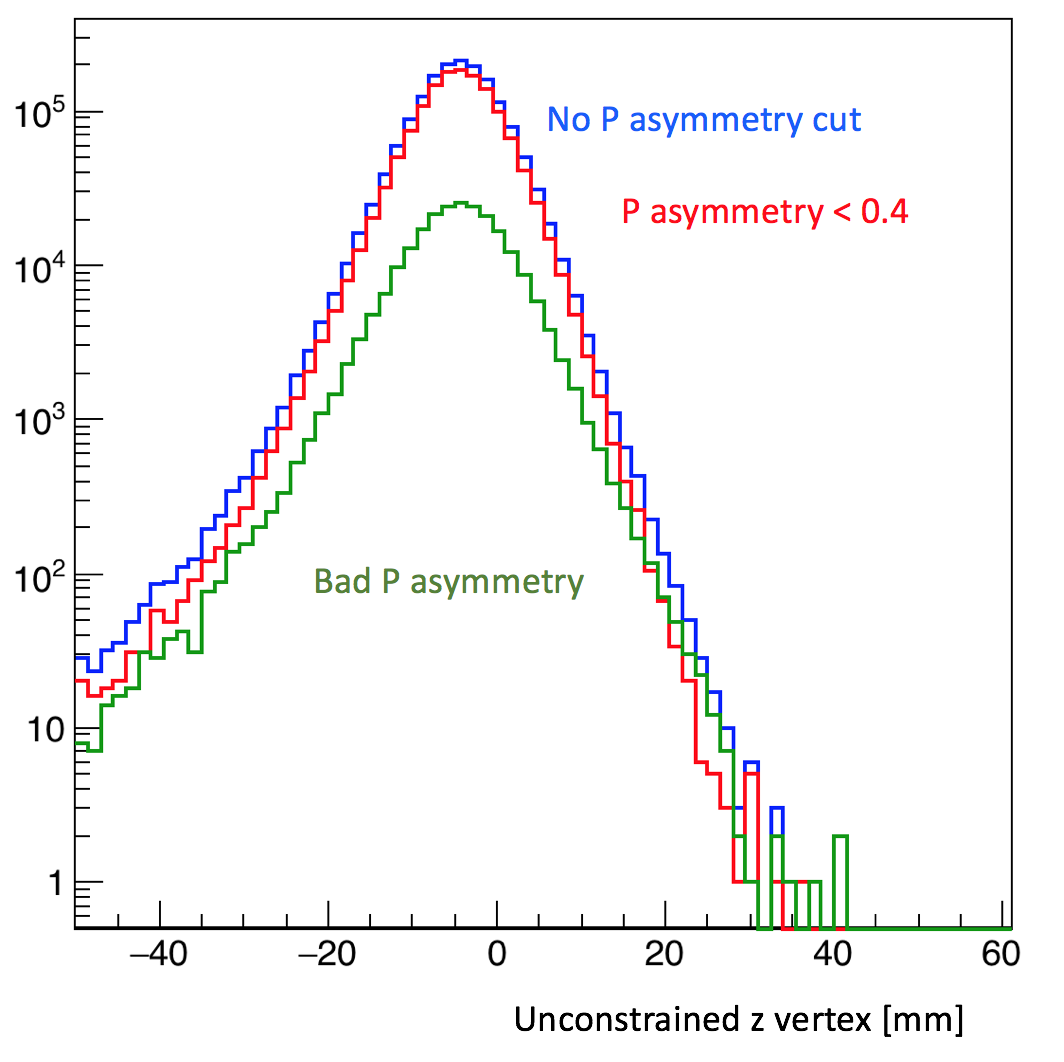
\includegraphics[width=0.5\textwidth]{pics/searching/pasycut.png}
  \caption[Cut on the momentum asymmetry]{The effect of the momentum asymmetry (the ratio of the momentum difference to the momentum sum of the two tracks) cut on the tails of the vertex distribution can be seen in the red an green curves.}
  \label{fig:pasycut}
\end{figure} 
The cut on the positron $DOCA$ is specifically intended to remove WAB contamination and downstream vertices from the pair-produced positron. The effects of the cut to the positron $DOCA$ on the vertex distribution are shown in Figure~\ref{fig:docacuteffect}. 
\begin{figure}[H]
  \centering
      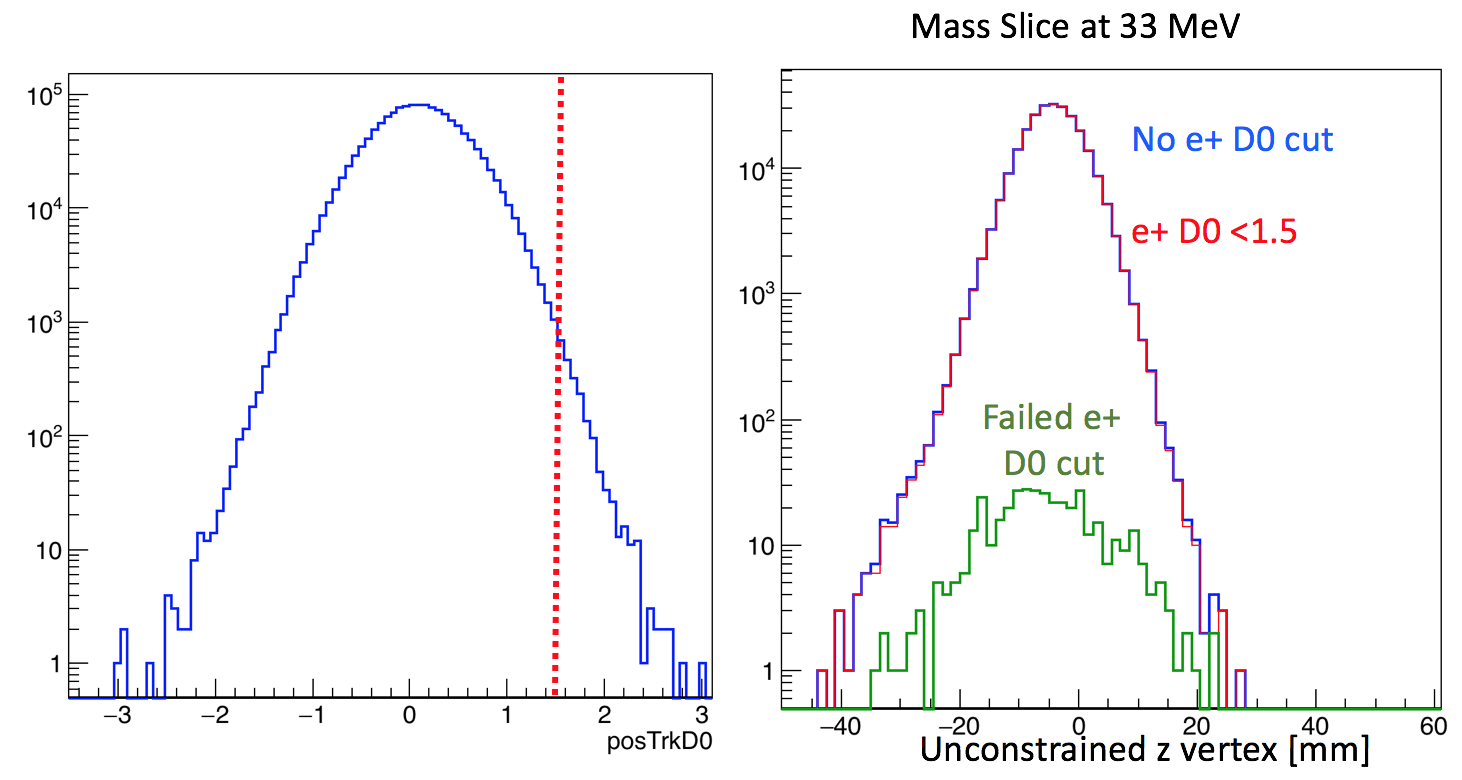
\includegraphics[width=0.75\textwidth]{pics/searching/docacut.png}
  \caption[Cut effect on the postiron $DOCA$]{Positrons that are produced from the photon in wide-angle bremsstrahlung events will have a distance of closest approach that will curve widely at the target location, yielding a largely positive value. The effects of the $DOCA$ cut on the vertex distribution is shown here.}
  \label{fig:docacuteffect}
\end{figure} 
Several downstream false vertices are produced that have a one hit difference with other tracks. Many of the tracks that share a lot of hits have nearly the same momentum as other tracks as shown in Figure~\ref{fig:trkshare}.
\begin{figure}[H]
  \centering
      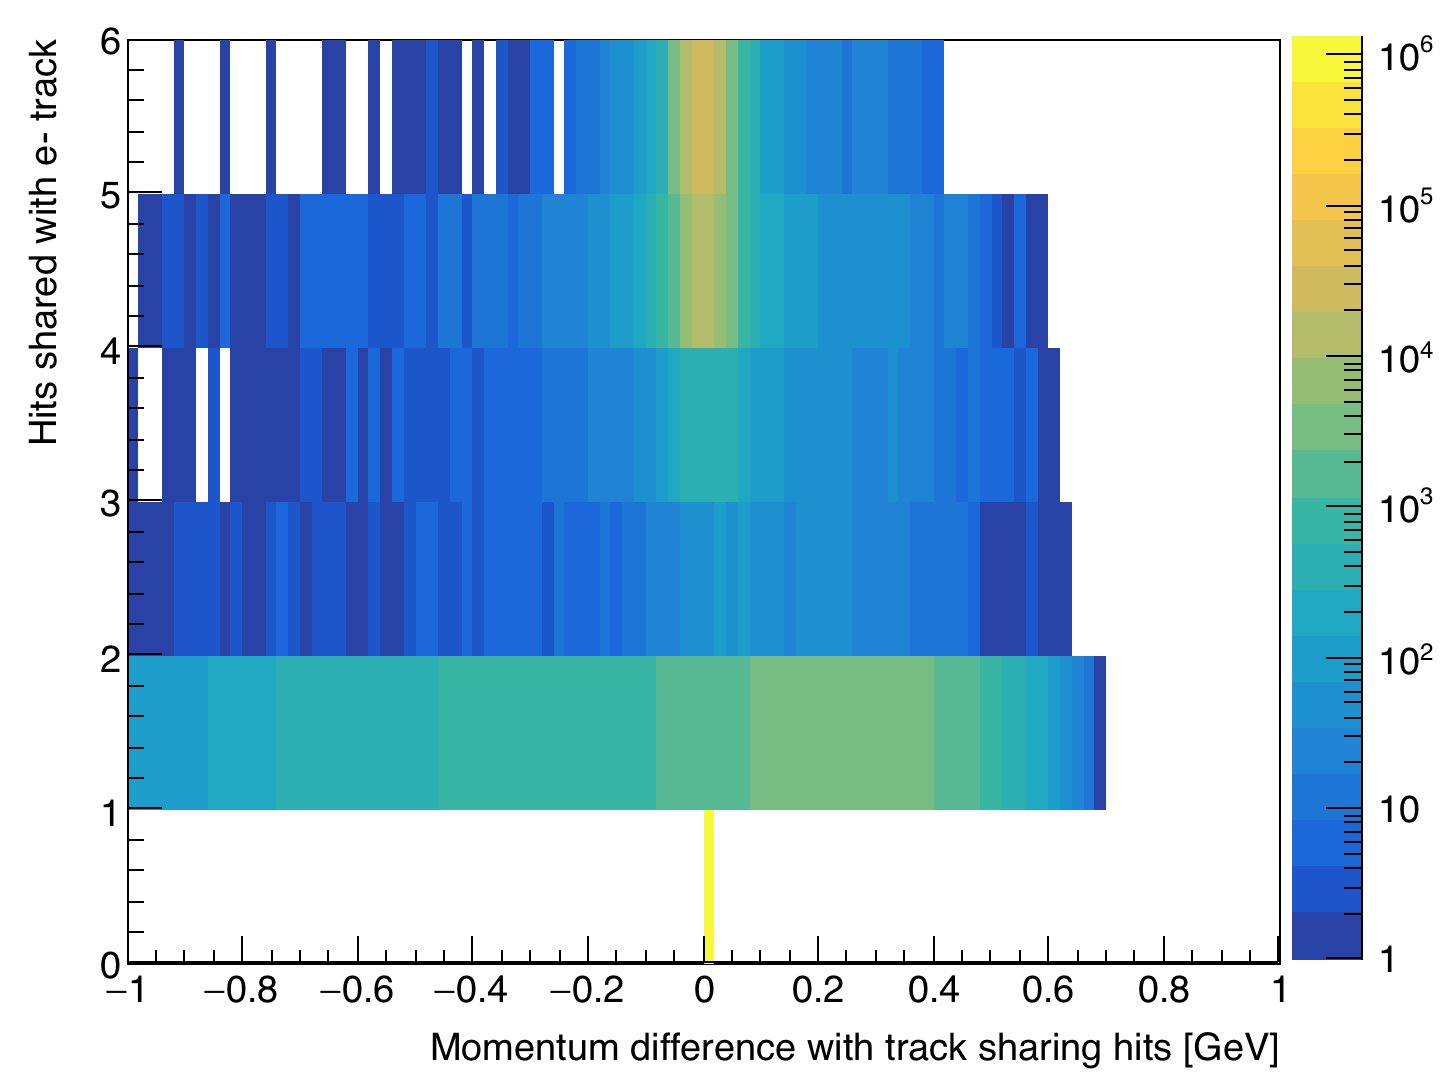
\includegraphics[width=0.5\textwidth]{pics/searching/TrkShareHits.png}
  \caption[Cut on shared hits between tracks]{This plot shows that many of the tracks sharing 4 and 5 hits with the initial track selected in the event have nearly the same momentum.}
  \label{fig:trkshare}
\end{figure} 

\subsection{L1L2 with SVT at 0.5 mm}

The L1L2 data set with the SVT at the nominal 0.5~mm position consists of tracks where the one track missed the active region of Layer 1. This data set combines the case for which the electron passes through Layer 1 and the positron passes through Layer 1 in order to obtaining the $zCut$ because it was noted that the tails of the distributions are the same (despite the known backgrounds being different and could merit improved cuts that would divide the data set in the future). \\
\indent The cuts applied to the L1L2 data set are shown in Table~\ref{l1l2_cuts}. 

\begin{table}[H]
\caption{Cuts applied to the L1L2 datasets.}
\label{l1l2_cuts}
\centering
\begin{tabular}{lllllll}
\toprule
%\multicolumn{2}{c}{Name} \\
%\cmidrule(r){1-2}
Cut type & Cut & Cut Value &  $\%$cut &  $\%$cut core & $\%$cut tails\\
\midrule
track & Fit quality & track $\chi^{2}<30$ & 38 & 15 & 47 \\
track & Max track momentum &  $P_{trk}<75\%E_{beam}$ & 12 & 8 & 14 \\
track & Isolation &   & 11 & 4 & 15 \\
vertex & beamspot constraint & bsc$\chi^{2}<10$  & 46 & 24 & 60 \\
vertex & beamspot - unconstrained & bsc$\chi^{2}$-unc$\chi^2<5$  & 20 & 16 & 24 \\
vertex & maximum $P_{sum}$ &  $<115\%E_{beam}$ & 1 & 1 & 1 \\
ecal & Ecal SVT matching & $\chi^2<10$  & 7 & 7 & 8 \\
ecal & track Ecal timing & $<4$ns  & 5 & 5 & 5 \\
ecal & 2 cluster time diff & $<2$ns  & 8 & 6 & 10 \\
physics & momentum asymmetry & $<0.4$  & 14 & 15 & 13 \\
physics & e+ track d0 & $<1.5$mm  & 7 & 3 & 11 \\
event & max shared hits amongst tracks & $<5$ shared hits  & 8 & 7 & 8 \\
track & cuts on kink tails & $\phi$ and $\lambda$ kink tails & 19 & 9 & 36 \\
\bottomrule
\end{tabular}
\end{table}

The initial selection requires that a track that missed Layer 1 has a projection to the $z$ location at layer 1 that is less than 1.5~mm from the beam. This ensures that the sample is not overly contaminated by events that passed through the active region but failed to identify a hit. As a result, the core of the distribution sits on the downstream side of the z-axis and reflects the geometric constraints we have imposed. The first cut that is different from the L1L1 data set is the isolation cut. In this data set, we apply the same isolation cut to the track that passed through Layer 1, but we apply a slightly different isolation cut for the track that did not pass through layer 1. The isolation in layer 2 is measured and projected to the target position to be compared with the impact parameter of the track in $y$ at the target. Additional cuts are applied to the tails of the kink distributions for the tracks. The summary of these cuts is made in the Table~\ref{kink_cuts}.

\begin{table}[H]
\caption{Cuts applied to the kinks in layers 1-3.}
\label{kink_cuts}
\centering
\begin{tabular}{lll}
\toprule
%\multicolumn{2}{c}{Name} \\
%\cmidrule(r){1-2}
Cut & Value \\
\midrule
Layer 1: $\phi$ kink, $\lambda$ kink & <0.0001,<0.002\\
Layer 2: $\phi$ kink, $\lambda$ kink & <0.002,<0.004\\
Layer 3: $\phi$ kink, $\lambda$ kink & <0.002,<0.004\\
\bottomrule
\end{tabular}
\end{table}

The uncut kink distributions for the electron with the cut indicated by the red dashed line is shown in Figures~\ref{fig:kink1}, \ref{fig:kink2}, and \ref{fig:kink3}.

\begin{figure}[H]
  \centering
      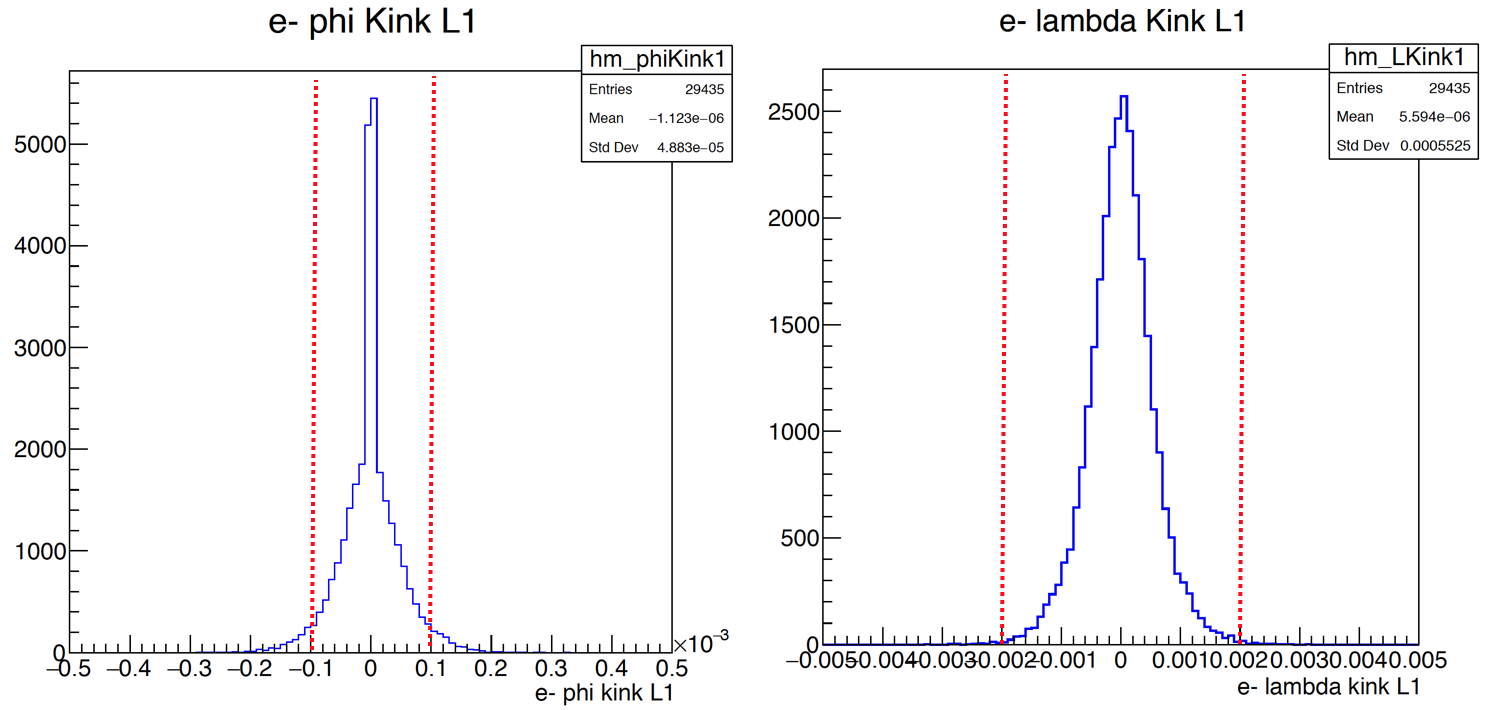
\includegraphics[width=0.8\textwidth]{pics/appendix/kink1.png}
  \caption[Kink distributions for Layer 1]{The kink distributions for tracks passing through Layer 1. The cut is shown at the red dashed line.}
  \label{fig:kink1}
\end{figure} 
\begin{figure}[H]
  \centering
      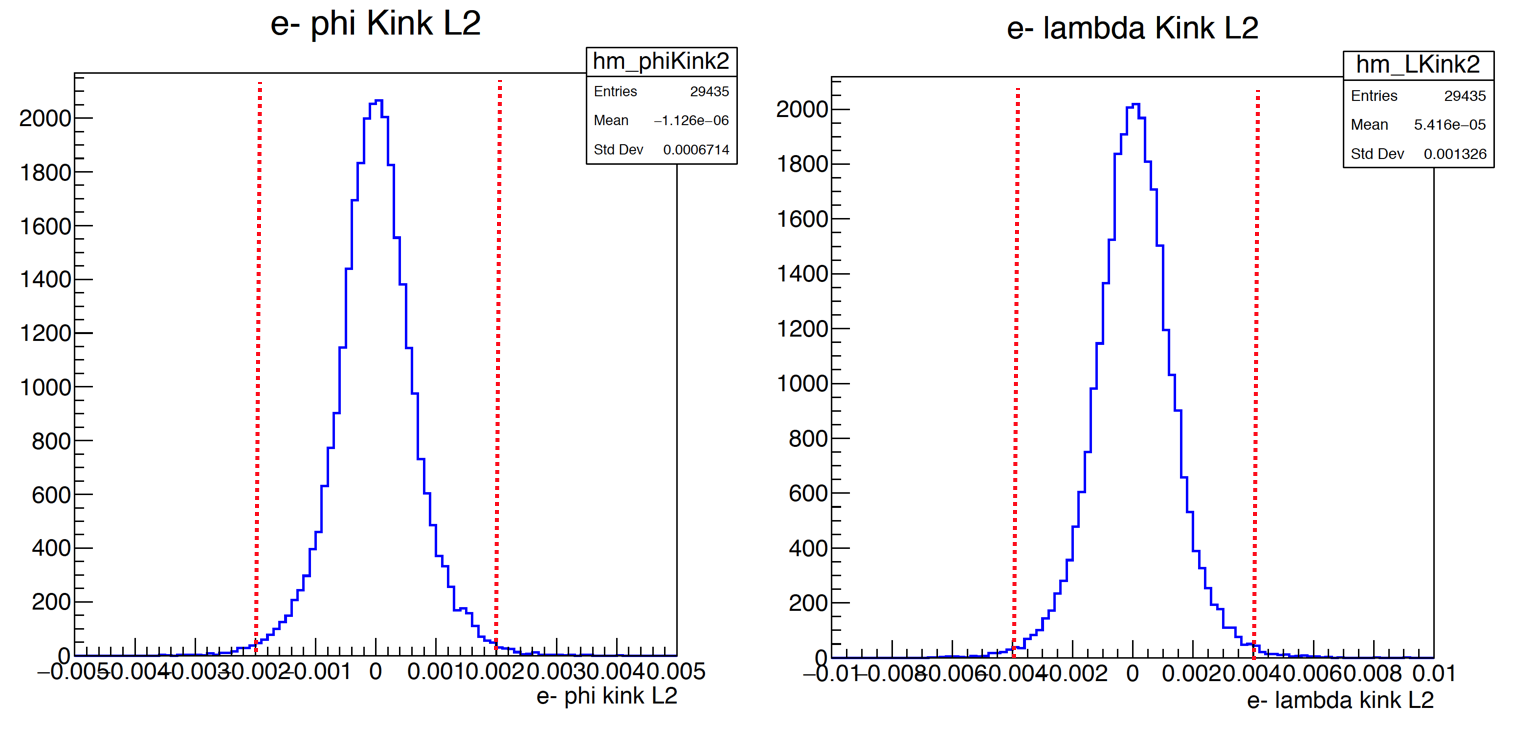
\includegraphics[width=0.8\textwidth]{pics/appendix/kink2.png}
  \caption[Kink distributions for Layer 2]{The kink distributions for tracks passing through Layer 2. The cut is shown at the red dashed line.}
  \label{fig:kink2}
\end{figure} 
\begin{figure}[H]
  \centering
      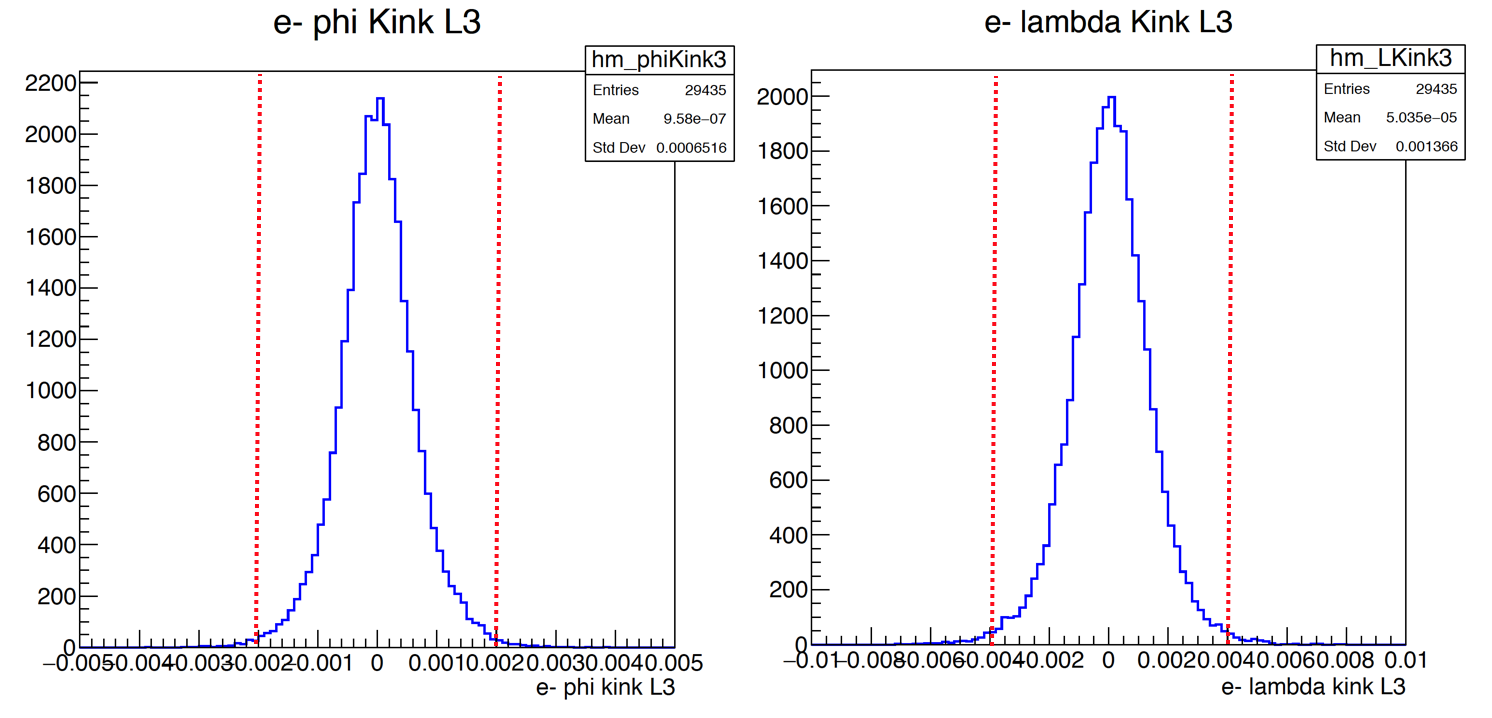
\includegraphics[width=0.8\textwidth]{pics/appendix/kink3.png}
  \caption[Kink distributions for Layer 3]{The kink distributions for tracks passing through Layer 3. The cut is shown at the red dashed line.}
  \label{fig:kink3}
\end{figure} 

The positron kink distributions look similar to the electron kink distributions and are not shown here. These cuts remove events from the tails. The effects of all the cuts on the reconstructed vertex position distribution are shown in Figure~\ref{fig:zvtxCuts_l1l2}.

\begin{figure}[H]
  \centering
      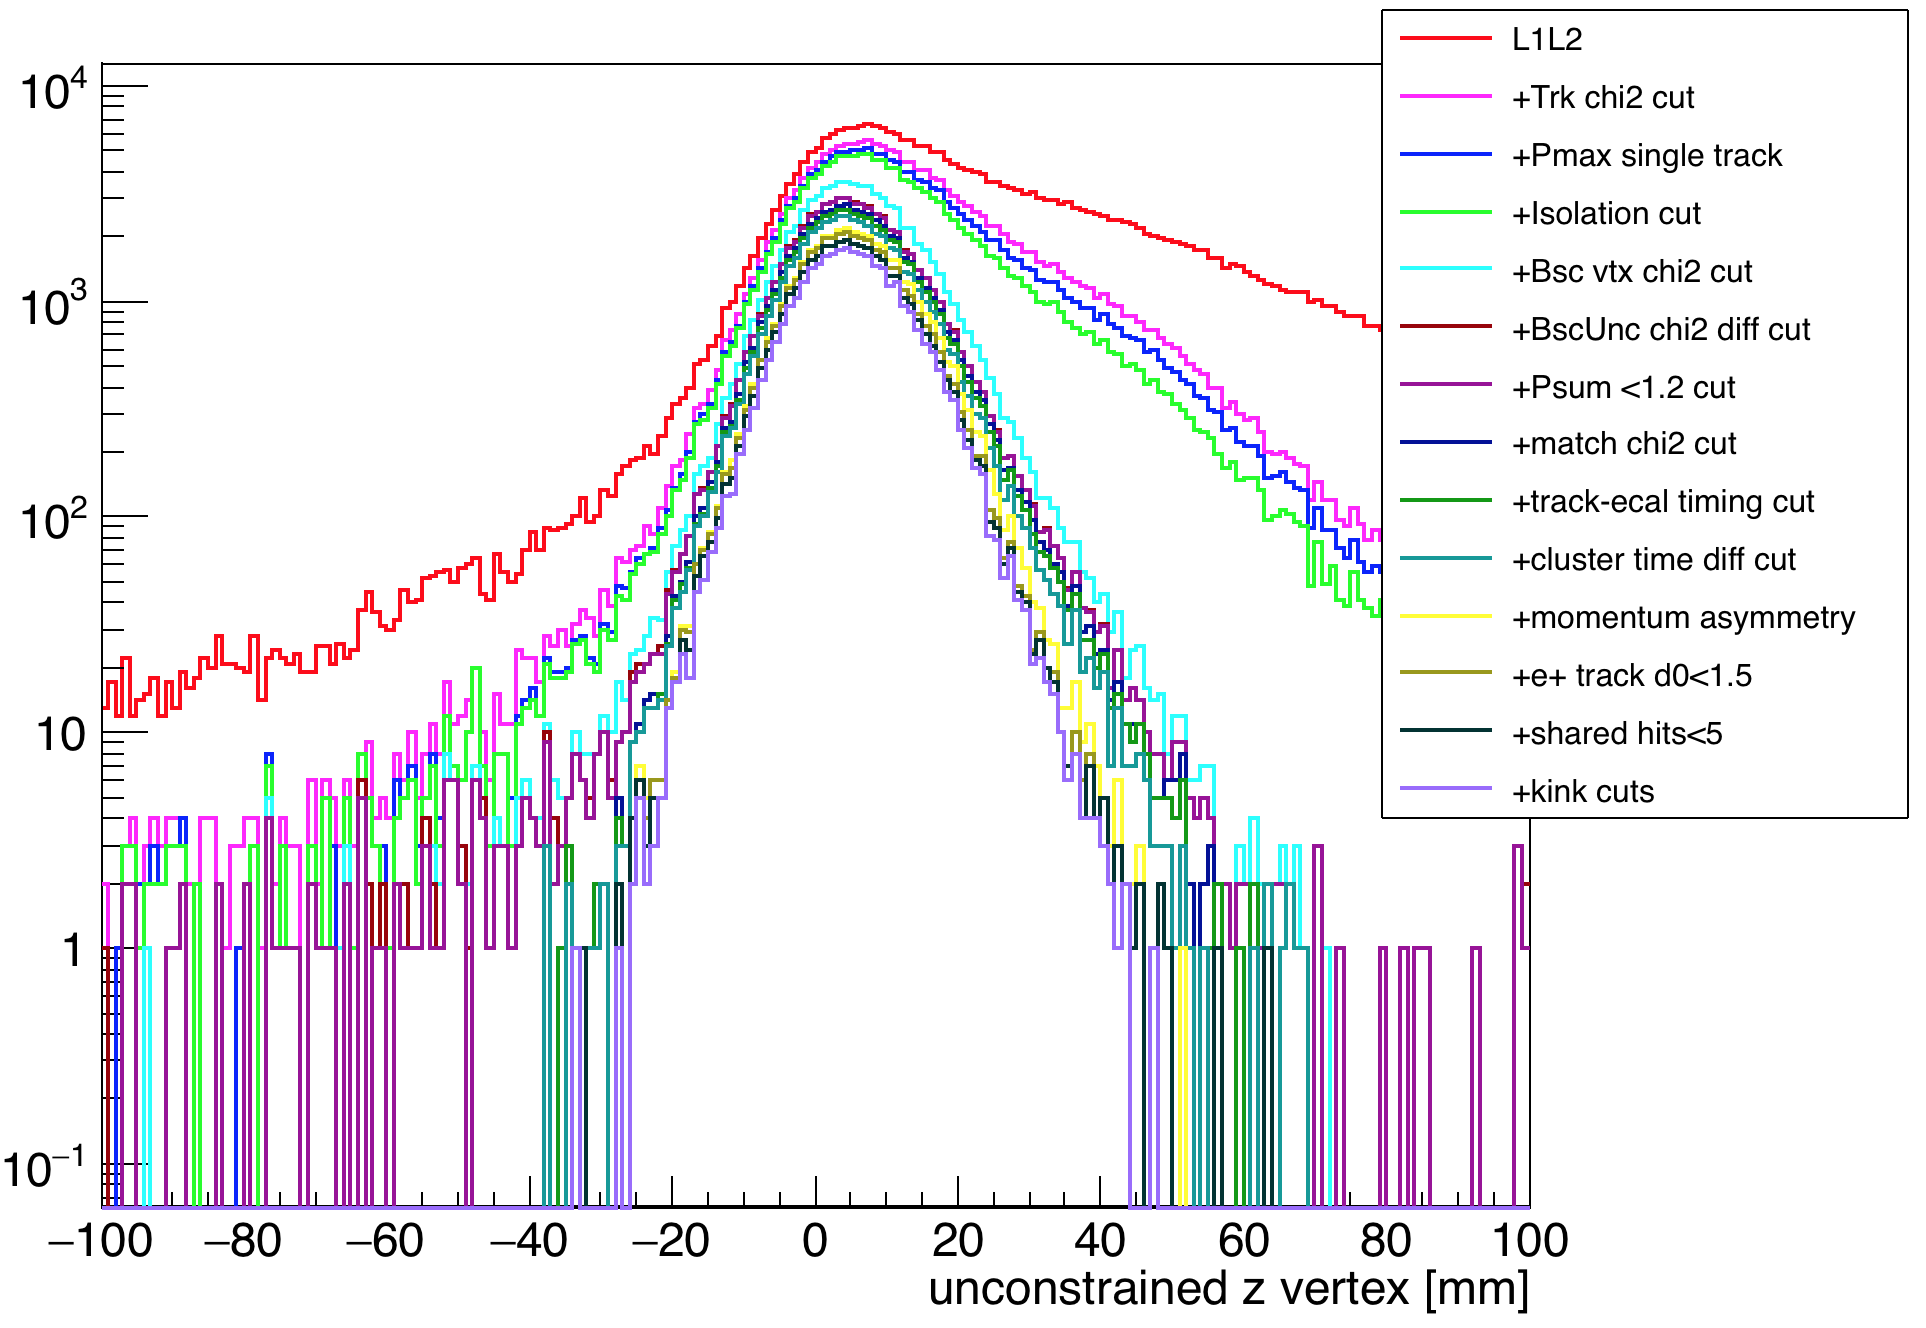
\includegraphics[width=0.8\textwidth]{pics/appendix/zvtxCuts_L1L2.png}
  \caption{The effects of the cuts on the L1L2 dataset on the unconstrained $z$ vertex.}
  \label{fig:zvtxCuts_l1l2}
\end{figure} 

The effects of the cuts on the reconstructed mass distribution are shown in Figure~\ref{fig:massCuts_l1l2}.

\begin{figure}[H]
  \centering
      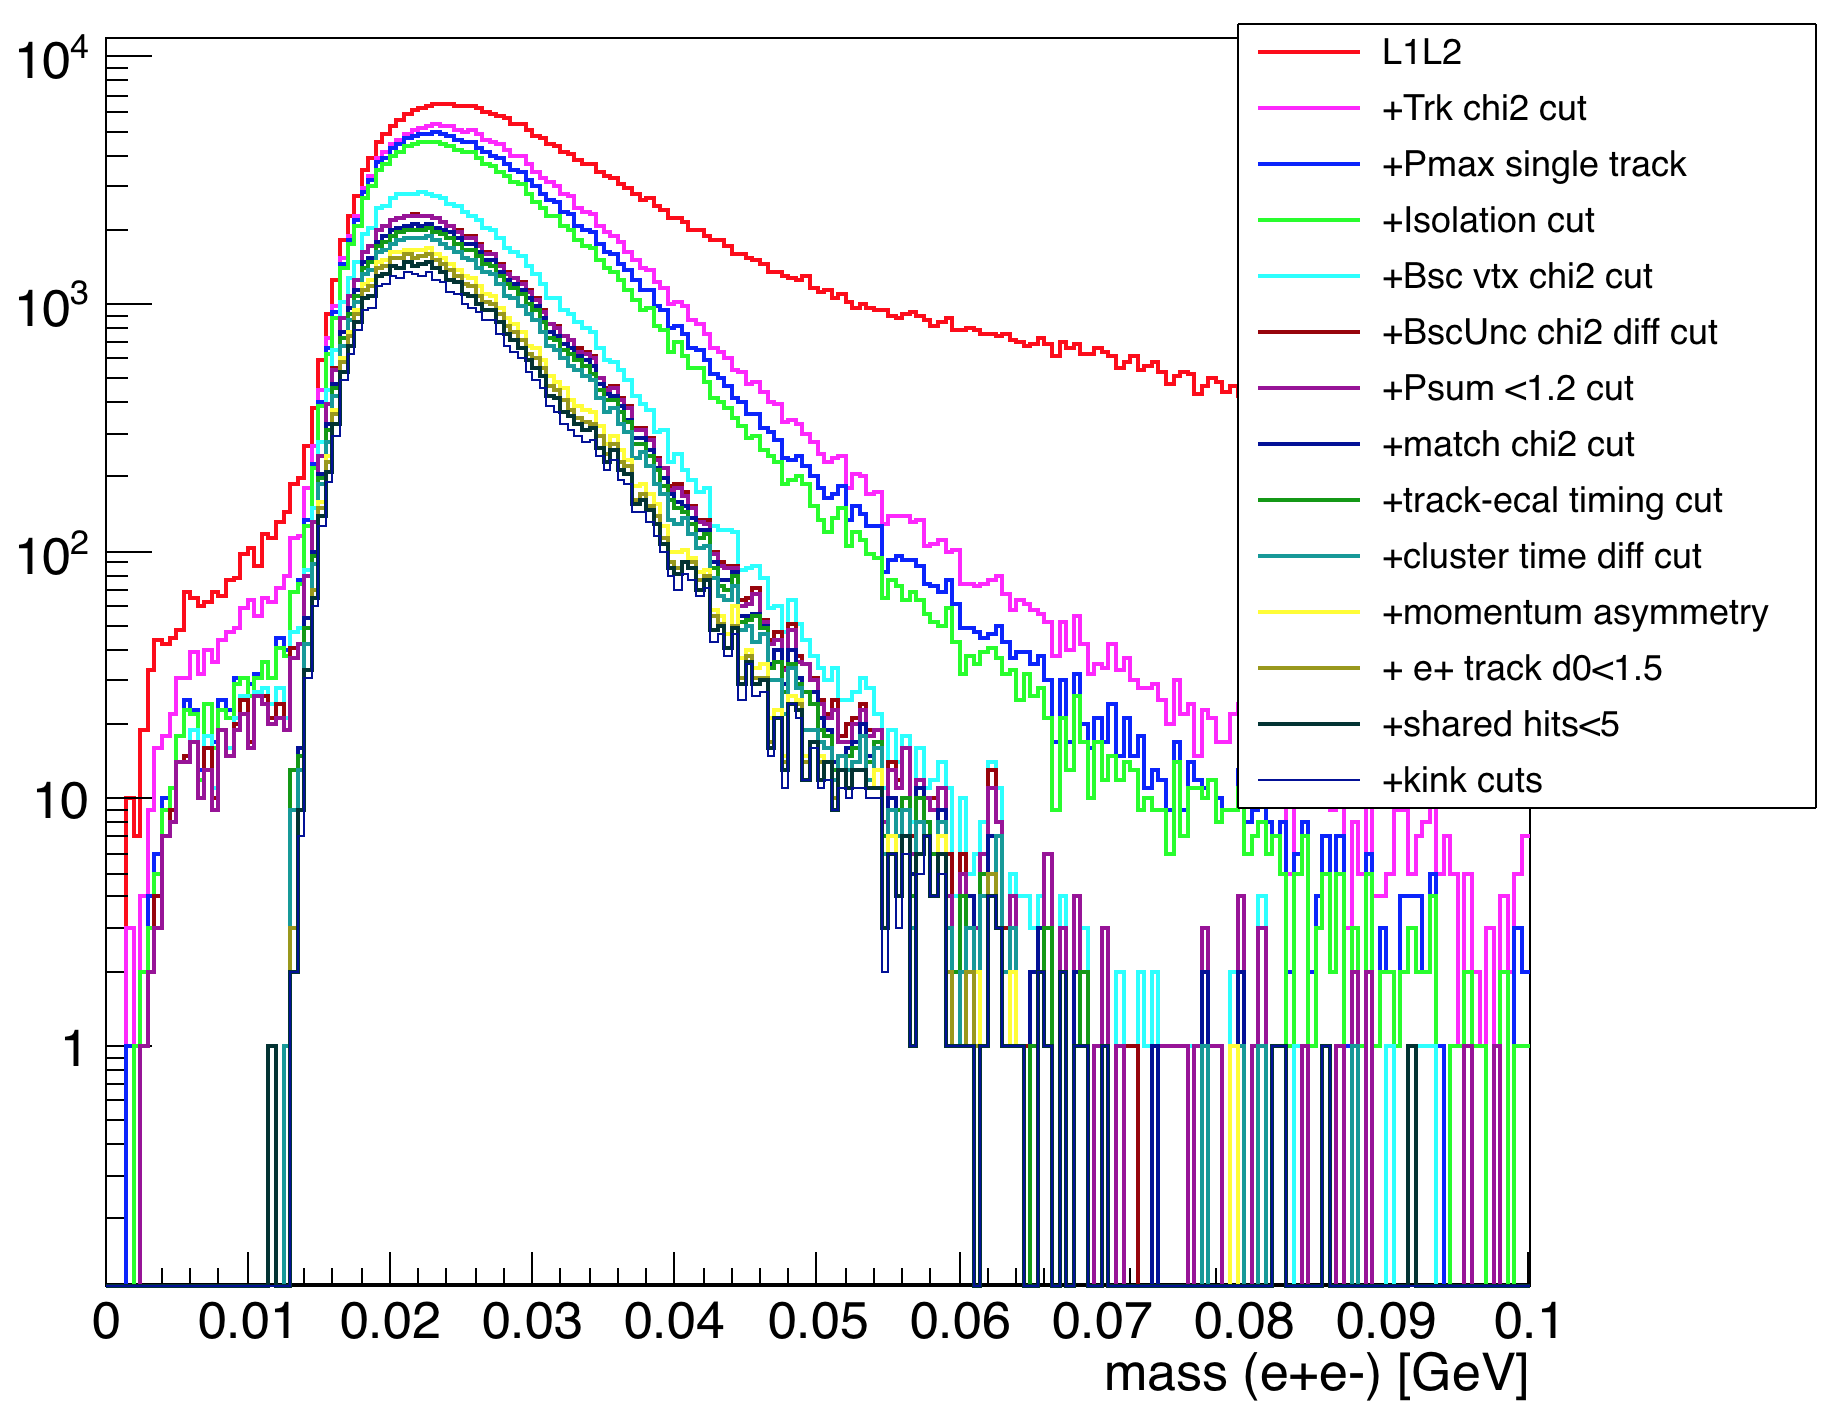
\includegraphics[width=0.8\textwidth]{pics/appendix/massCuts_L1L2.png}
  \caption{The effects of the cuts on the L1L2 data set on the mass distribution.}
  \label{fig:massCuts_l1l2}
\end{figure} 

This dataset has the tendency to contain more WAB contamination than the L1L1 data set. In particular, we know from Monte Carlo that positrons are unlikely to have a hit in Layer 1 when the photon in WAB pair produces after the target. Additionally, this sample contains a 5:1 ratio of having in electron versus a positron in the first layer. 

\subsection{L2L2 with SVT at 0.5 mm}

The L2L2 dataset consists of vertices produced when tracks do not pass through Layer 1 and their projections back to Layer 1 are within 1.5~mm of the beam (outside the active silicon region). This data set requires the most work to remove the background events, and preliminary studies with the small number of statistics have been unsuccessful. \\
\indent The general cuts applied to the L2L2 data set, after first requiring that track projections do not extend to the active region of Layer 1, are listed in Table~\ref{l2l2_cuts}.

\begin{table}[H]
\caption{Cuts applied to the L2L2 data sets.}
\label{l2l2_cuts}
\centering
\begin{tabular}{lllllll}
\toprule
%\multicolumn{2}{c}{Name} \\
%\cmidrule(r){1-2}
Cut type & Cut & Cut Value &  $\%$cut &  $\%$cut core & $\%$cut tails\\
\midrule
track & Fit quality & track $\chi^{2}<30$ & 44 & 66 & 44 \\
track & Max track momentum &  $P_{trk}<75\%E_{beam}$ & 15 & 14 & 15 \\
track & Isolation &   & 22 & 34 & 22 \\
vertex & beamspot constraint & bsc$\chi^{2}<10$  & 47 & 36 & 47 \\
vertex & beamspot - unconstrained & bsc$\chi^{2}$-unc$\chi^2<5$  & 18 & 0 & 19 \\
vertex & maximum $P_{sum}$ &  $<115\%E_{beam}$ & 1 & 6 & 1 \\
ecal & Ecal SVT matching & $\chi^2<10$  & 30 & 73 & 29 \\
ecal & track Ecal timing & $<4$ns  & 7 & 0 & 8 \\
ecal & 2 cluster time diff & $<2$ns  & 8 & 0 & 8 \\
physics & momentum asymmetry & $<0.4$  & 4 & 0 & 4 \\
physics & e+ track d0 & $<1.5$mm  & 21 & 33 & 21 \\
event & max shared hits amongst tracks & $<4$ shared hits  & 21 & 50 & 21 \\
\bottomrule
\end{tabular}
\end{table}

The geometric acceptance of the cuts in the L2L2 data set leave a core fraction of background events well beyond the target at approximately 30~mm downstream. The only modifications to previously applied cuts are that both tracks use a modified isolation cut by looking at the isolation at Layer 2 and the tracks do not share 4 hits with any other track in the event.  The kink cuts appeared to not remove events from this data set.

\subsection{L1L1 with SVT at 1.5 mm}
The L1L1 data set in the 1.5~mm data includes vertices reconstructed from pairs of tracks that have hits in Layer 1 of the SVT. Due to the SVT opening being larger, the acceptance favors larger heavy photon masses. The SVT has also lower rates in Layer 1 when compared to the 0.5~mm data set.\\
\indent The cuts applied to the L1L1 data set are shown in Table~\ref{l1l1_cuts_1p5}.

\begin{table}[H]
\caption{Cuts applied to the L1L1 data sets with the SVT at 1.5mm.}
\label{l1l1_cuts_1p5}
\centering
\begin{tabular}{llllll}
\toprule
%\multicolumn{2}{c}{Name} \\
%\cmidrule(r){1-2}
Cut type & Cut & Cut Value &  $\%$cut &  $\%$cut core & $\%$cut tails\\
\midrule
track & Fit quality & track $\chi^{2}<30$ & 37 & 22 & 87 \\
track & Max track momentum &  $P_{trk}<75\%E_{beam}$ & 6 & 6 & 19 \\
track & Isolation &   & 2 & 1 & 15 \\
vertex & beamspot constraint & bsc$\chi^{2}<10$  & 23 & 21 & 81 \\
vertex & beamspot - unconstrained & bsc$\chi^{2}$-unc$\chi^2<5$  & 12 & 12 & 27 \\
vertex & maximum $P_{sum}$ &  $<115\%E_{beam}$ & 0 & 0 & 2 \\
ecal & Ecal SVT matching & $\chi^2<10$  & 3 & 3 & 58 \\
ecal & track Ecal timing & $<4$ns  & 5 & 5 & 7 \\
ecal & 2 cluster time diff & $<2$ns  & 4 & 4 & 13 \\
physics & momentum asymmetry & $<0.4$  & 12 & 12 & 48 \\
physics & e+ track d0 & $<1.5$mm  & 0 & 0 & 4 \\
event & max shared hits amongst tracks & $<5$ shared hits  & 12 & 12 & 20 \\
\bottomrule
\end{tabular}
\end{table}

The cuts are the same as those applied to the 0.5~mm data set with similar effect.

\subsection{L1L2 with SVT at 1.5 mm}
The following section describes the data set where one track misses Layer 1 of the SVT and its track projection back to Layer 1 is within 2.5~mm of the beam such that the track does not extrapolate to the active region of the silicon.\\
\indent The cuts applied to the L1L2 dataset with the first layer of the SVT at 1.5~mm is shown in Table~\ref{l1l2_cuts_1p5}.

\begin{table}[H]
\caption{Cuts applied to the L1L2 data sets with the SVT at 1.5~mm.}
\label{l1l2_cuts_1p5}
\centering
\begin{tabular}{lllllll}
\toprule
%\multicolumn{2}{c}{Name} \\
%\cmidrule(r){1-2}
Cut type & Cut & Cut Value &  $\%$cut &  $\%$cut core & $\%$cut tails\\
\midrule
track & Fit quality & track $\chi^{2}<30$ & 23 & 11 & 47 \\
track & Max track momentum &  $P_{trk}<75\%E_{beam}$ & 8 & 7 & 12 \\
track & Isolation &   & 4 & 2 & 10 \\
vertex & beamspot constraint & bsc$\chi^{2}<10$  & 29 & 20 & 62 \\
vertex & beamspot - unconstrained & bsc$\chi^{2}$-unc$\chi^2<5$  & 12 & 11 & 22 \\
vertex & maximum $P_{sum}$ &  $<115\%E_{beam}$ & 0 & 0 & 0 \\
ecal & Ecal SVT matching & $\chi^2<10$  & 5 & 5 & 7 \\
ecal & track Ecal timing & $<4$ns  & 5 & 5 & 5 \\
ecal & 2 cluster time diff & $<2$ns  & 6 & 5 & 9 \\
physics & momentum asymmetry & $<0.4$  & 14 & 13 & 16 \\
physics & e+ track d0 & $<1.5$mm  & 6 & 5 & 16 \\
event & max shared hits amongst tracks & $<5$ shared hits  & 6 & 6 & 6 \\
track & cuts on kink tails & $\phi$ and $\lambda$ kink tails & 22 & 8 & 74 \\
\bottomrule
\end{tabular}
\end{table}

The cuts applied to the L1L2 data set may require a similar optimization to eliminate backgrounds as that required of the data set for the 0.5~mm. Namely, that, it may be necessary to separate the data set for events where the positron versus the electron is the first to leave a hit in Layer 1. For the moment, the same cuts are used as the 1.5~mm data set has generally lower backgrounds than that seen in the 0.5~mm data set.

\subsection{L2L2 with SVT at 1.5 mm}
The following section discusses the events having no hit in Layer 1 of the 1.5~mm data set. An additional requirement was made that the tracks must not project back to the active region of the Layer 1 silicon in order to avoid contamination by events with the Layer 1 inefficiency. \\
\indent The cuts applied to the L2L2 data set are shown in Table~\ref{l2l2_cuts_1p5}.

\begin{table}[H]
\caption{Cuts applied to the L2L2 data sets with the SVT at 1.5~mm.}
\label{l2l2_cuts_1p5}
\centering
\begin{tabular}{lllllll}
\toprule
%\multicolumn{2}{c}{Name} \\
%\cmidrule(r){1-2}
Cut type & Cut & Cut Value &  $\%$cut &  $\%$cut core & $\%$cut tails\\
\midrule
track & Fit quality & track $\chi^{2}<30$ & 29 & 11 & 39 \\
track & Max track momentum &  $P_{trk}<75\%E_{beam}$ & 10 & 8 & 12 \\
track & Isolation &   & 5 & 2 & 8 \\
vertex & beamspot constraint & bsc$\chi^{2}<10$  & 26 & 16 & 35 \\
vertex & beamspot - unconstrained & bsc$\chi^{2}$-unc$\chi^2<5$  & 10 & 8 & 14 \\
vertex & maximum $P_{sum}$ &  $<115\%E_{beam}$ & 1 & 1 & 1 \\
ecal & Ecal SVT matching & $\chi^2<10$  & 11 & 8 & 14 \\
ecal & track Ecal timing & $<4$ns  & 6 & 6 & 6 \\
ecal & 2 cluster time diff & $<2$ns  & 7 & 6 & 7 \\
physics & momentum asymmetry & $<0.4$  & 3 & 2 & 4 \\
physics & e+ track d0 & $<1.5$mm  & 9 & 7 & 12 \\
event & max shared hits amongst tracks & $<4$ shared hits  & 20 & 20 & 20 \\
\bottomrule
\end{tabular}
\end{table}

The cuts are the same as those applied to the data in the 0.5~mm L2L2 data set. This data set has significantly more statistics that needs to be studied and may complement the analysis on the 0.5~mm high $z$ background data. 